\documentclass[1p]{elsarticle_modified}
%\bibliographystyle{elsarticle-num}

%\usepackage[colorlinks]{hyperref}
%\usepackage{abbrmath_seonhwa} %\Abb, \Ascr, \Acal ,\Abf, \Afrak
\usepackage{amsfonts}
\usepackage{amssymb}
\usepackage{amsmath}
\usepackage{amsthm}
\usepackage{scalefnt}
\usepackage{amsbsy}
\usepackage{kotex}
\usepackage{caption}
\usepackage{subfig}
\usepackage{color}
\usepackage{graphicx}
\usepackage{xcolor} %% white, black, red, green, blue, cyan, magenta, yellow
\usepackage{float}
\usepackage{setspace}
\usepackage{hyperref}

\usepackage{tikz}
\usetikzlibrary{arrows}

\usepackage{multirow}
\usepackage{array} % fixed length table
\usepackage{hhline}

%%%%%%%%%%%%%%%%%%%%%
\makeatletter
\renewcommand*\env@matrix[1][\arraystretch]{%
	\edef\arraystretch{#1}%
	\hskip -\arraycolsep
	\let\@ifnextchar\new@ifnextchar
	\array{*\c@MaxMatrixCols c}}
\makeatother %https://tex.stackexchange.com/questions/14071/how-can-i-increase-the-line-spacing-in-a-matrix
%%%%%%%%%%%%%%%

\usepackage[normalem]{ulem}

\newcommand{\msout}[1]{\ifmmode\text{\sout{\ensuremath{#1}}}\else\sout{#1}\fi}
%SOURCE: \msout is \stkout macro in https://tex.stackexchange.com/questions/20609/strikeout-in-math-mode

\newcommand{\cancel}[1]{
	\ifmmode
	{\color{red}\msout{#1}}
	\else
	{\color{red}\sout{#1}}
	\fi
}

\newcommand{\add}[1]{
	{\color{blue}\uwave{#1}}
}

\newcommand{\replace}[2]{
	\ifmmode
	{\color{red}\msout{#1}}{\color{blue}\uwave{#2}}
	\else
	{\color{red}\sout{#1}}{\color{blue}\uwave{#2}}
	\fi
}

\newcommand{\Sol}{\mathcal{S}} %segment
\newcommand{\D}{D} %diagram
\newcommand{\A}{\mathcal{A}} %arc


%%%%%%%%%%%%%%%%%%%%%%%%%%%%%5 test

\def\sl{\operatorname{\textup{SL}}(2,\Cbb)}
\def\psl{\operatorname{\textup{PSL}}(2,\Cbb)}
\def\quan{\mkern 1mu \triangleright \mkern 1mu}

\theoremstyle{definition}
\newtheorem{thm}{Theorem}[section]
\newtheorem{prop}[thm]{Proposition}
\newtheorem{lem}[thm]{Lemma}
\newtheorem{ques}[thm]{Question}
\newtheorem{cor}[thm]{Corollary}
\newtheorem{defn}[thm]{Definition}
\newtheorem{exam}[thm]{Example}
\newtheorem{rmk}[thm]{Remark}
\newtheorem{alg}[thm]{Algorithm}

\newcommand{\I}{\sqrt{-1}}
\begin{document}

%\begin{frontmatter}
%
%\title{Boundary parabolic representations of knots up to 8 crossings}
%
%%% Group authors per affiliation:
%\author{Yunhi Cho} 
%\address{Department of Mathematics, University of Seoul, Seoul, Korea}
%\ead{yhcho@uos.ac.kr}
%
%
%\author{Seonhwa Kim} %\fnref{s_kim}}
%\address{Center for Geometry and Physics, Institute for Basic Science, Pohang, 37673, Korea}
%\ead{ryeona17@ibs.re.kr}
%
%\author{Hyuk Kim}
%\address{Department of Mathematical Sciences, Seoul National University, Seoul 08826, Korea}
%\ead{hyukkim@snu.ac.kr}
%
%\author{Seokbeom Yoon}
%\address{Department of Mathematical Sciences, Seoul National University, Seoul, 08826,  Korea}
%\ead{sbyoon15@snu.ac.kr}
%
%\begin{abstract}
%We find all boundary parabolic representation of knots up to 8 crossings.
%
%\end{abstract}
%\begin{keyword}
%    \MSC[2010] 57M25 
%\end{keyword}
%
%\end{frontmatter}

%\linenumbers
%\tableofcontents
%
\newcommand\colored[1]{\textcolor{white}{\rule[-0.35ex]{0.8em}{1.4ex}}\kern-0.8em\color{red} #1}%
%\newcommand\colored[1]{\textcolor{white}{ #1}\kern-2.17ex	\textcolor{white}{ #1}\kern-1.81ex	\textcolor{white}{ #1}\kern-2.15ex\color{red}#1	}

{\Large $\underline{12n_{0767}~(K12n_{0767})}$}

\setlength{\tabcolsep}{10pt}
\renewcommand{\arraystretch}{1.6}
\vspace{1cm}\begin{tabular}{m{100pt}>{\centering\arraybackslash}m{274pt}}
\multirow{5}{120pt}{
	\centering
	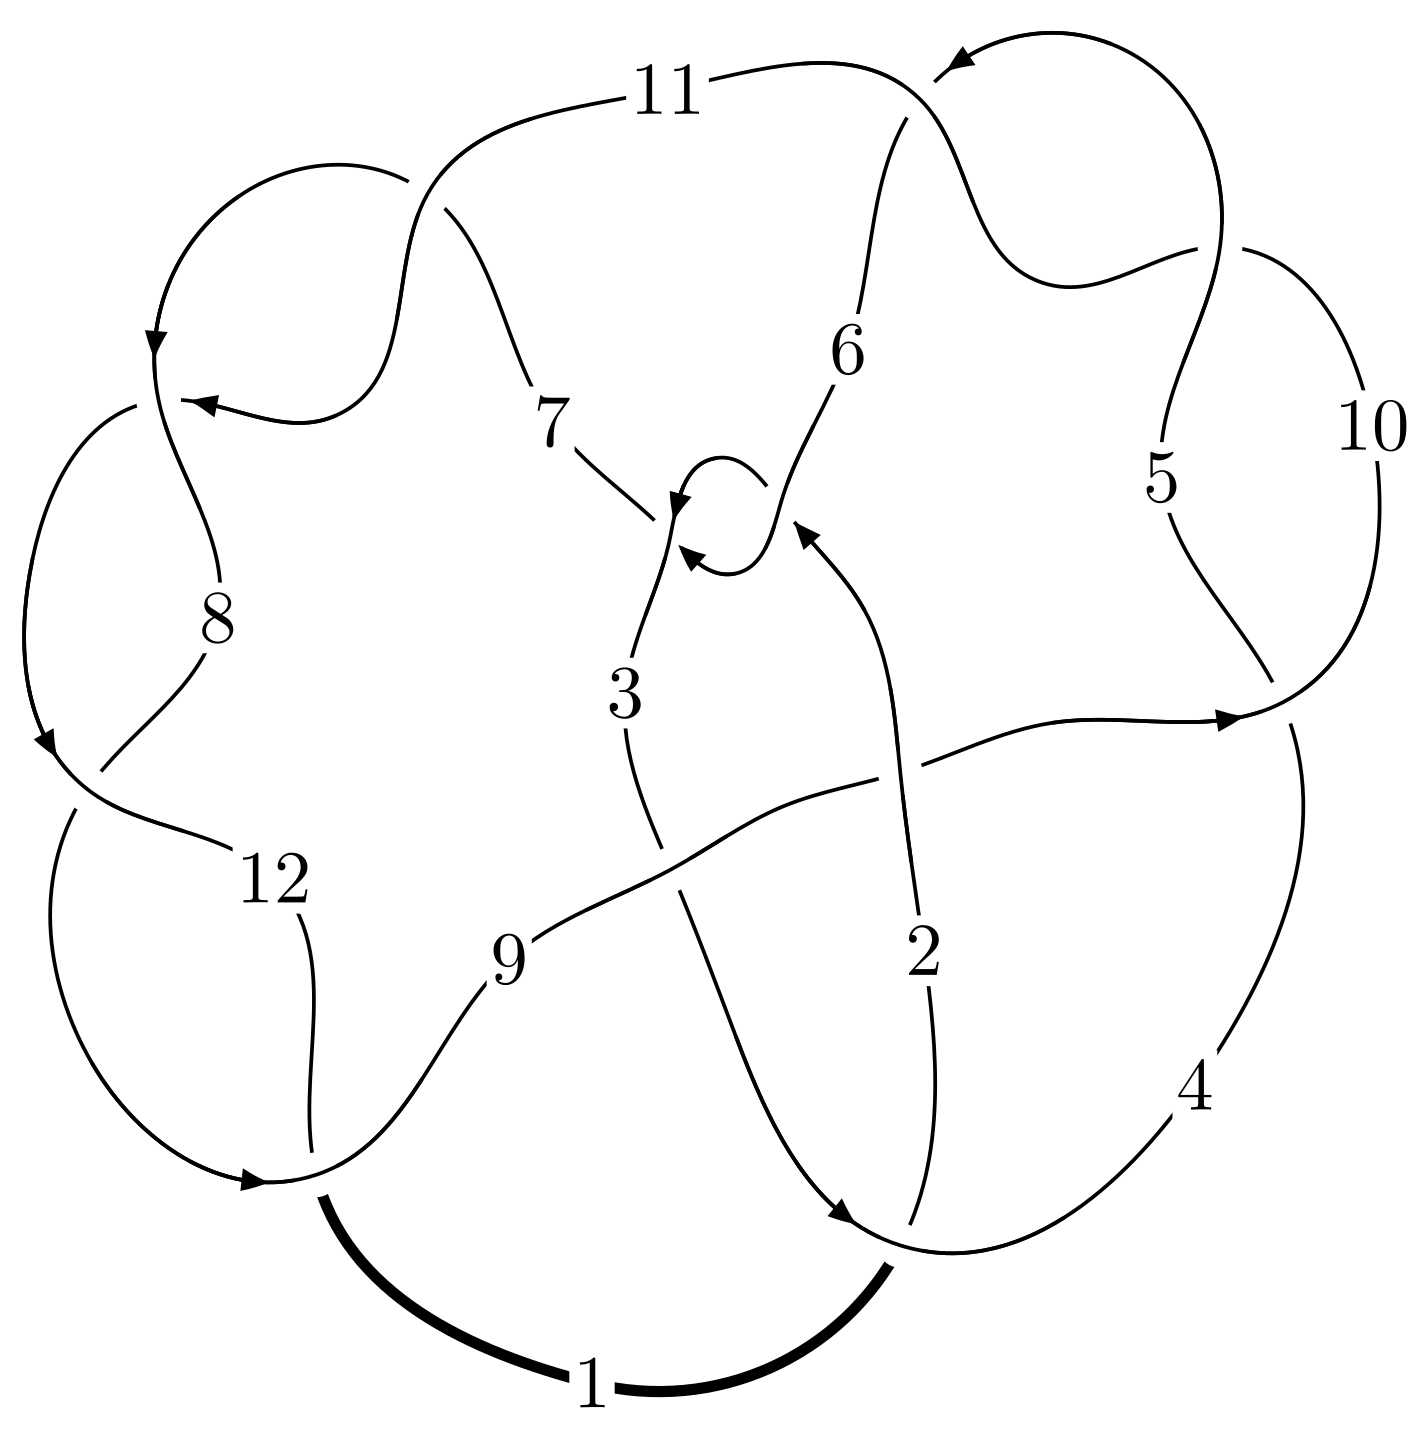
\includegraphics[width=112pt]{../../../GIT/diagram.site/Diagrams/png/2856_12n_0767.png}\\
\ \ \ A knot diagram\footnotemark}&
\allowdisplaybreaks
\textbf{Linearized knot diagam} \\
\cline{2-2}
 &
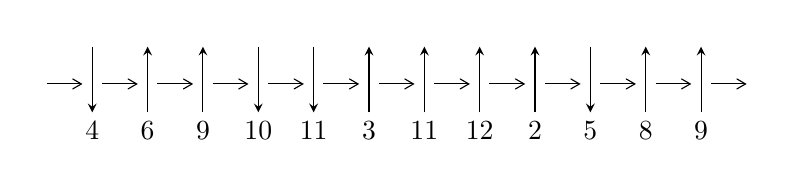
\begin{tikzpicture}[x=20pt, y=17pt]
	% nodes
	\node (C0) at (0, 0) {};
	\node (C1) at (1, 0) {};
	\node (C1U) at (1, +1) {};
	\node (C1D) at (1, -1) {4};

	\node (C2) at (2, 0) {};
	\node (C2U) at (2, +1) {};
	\node (C2D) at (2, -1) {6};

	\node (C3) at (3, 0) {};
	\node (C3U) at (3, +1) {};
	\node (C3D) at (3, -1) {9};

	\node (C4) at (4, 0) {};
	\node (C4U) at (4, +1) {};
	\node (C4D) at (4, -1) {10};

	\node (C5) at (5, 0) {};
	\node (C5U) at (5, +1) {};
	\node (C5D) at (5, -1) {11};

	\node (C6) at (6, 0) {};
	\node (C6U) at (6, +1) {};
	\node (C6D) at (6, -1) {3};

	\node (C7) at (7, 0) {};
	\node (C7U) at (7, +1) {};
	\node (C7D) at (7, -1) {11};

	\node (C8) at (8, 0) {};
	\node (C8U) at (8, +1) {};
	\node (C8D) at (8, -1) {12};

	\node (C9) at (9, 0) {};
	\node (C9U) at (9, +1) {};
	\node (C9D) at (9, -1) {2};

	\node (C10) at (10, 0) {};
	\node (C10U) at (10, +1) {};
	\node (C10D) at (10, -1) {5};

	\node (C11) at (11, 0) {};
	\node (C11U) at (11, +1) {};
	\node (C11D) at (11, -1) {8};

	\node (C12) at (12, 0) {};
	\node (C12U) at (12, +1) {};
	\node (C12D) at (12, -1) {9};
	\node (C13) at (13, 0) {};

	% arrows
	\draw[->,>={angle 60}]
	(C0) edge (C1) (C1) edge (C2) (C2) edge (C3) (C3) edge (C4) (C4) edge (C5) (C5) edge (C6) (C6) edge (C7) (C7) edge (C8) (C8) edge (C9) (C9) edge (C10) (C10) edge (C11) (C11) edge (C12) (C12) edge (C13) ;	\draw[->,>=stealth]
	(C1U) edge (C1D) (C2D) edge (C2U) (C3D) edge (C3U) (C4U) edge (C4D) (C5U) edge (C5D) (C6D) edge (C6U) (C7D) edge (C7U) (C8D) edge (C8U) (C9D) edge (C9U) (C10U) edge (C10D) (C11D) edge (C11U) (C12D) edge (C12U) ;
	\end{tikzpicture} \\
\hhline{~~} \\& 
\textbf{Solving Sequence} \\ \cline{2-2} 
 &
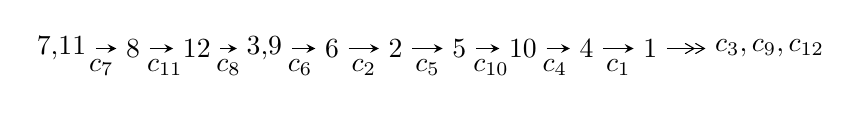
\begin{tikzpicture}[x=23pt, y=7pt]
	% node
	\node (A0) at (-1/8, 0) {7,11};
	\node (A1) at (1, 0) {8};
	\node (A2) at (2, 0) {12};
	\node (A3) at (49/16, 0) {3,9};
	\node (A4) at (33/8, 0) {6};
	\node (A5) at (41/8, 0) {2};
	\node (A6) at (49/8, 0) {5};
	\node (A7) at (57/8, 0) {10};
	\node (A8) at (65/8, 0) {4};
	\node (A9) at (73/8, 0) {1};
	\node (C1) at (1/2, -1) {$c_{7}$};
	\node (C2) at (3/2, -1) {$c_{11}$};
	\node (C3) at (5/2, -1) {$c_{8}$};
	\node (C4) at (29/8, -1) {$c_{6}$};
	\node (C5) at (37/8, -1) {$c_{2}$};
	\node (C6) at (45/8, -1) {$c_{5}$};
	\node (C7) at (53/8, -1) {$c_{10}$};
	\node (C8) at (61/8, -1) {$c_{4}$};
	\node (C9) at (69/8, -1) {$c_{1}$};
	\node (A10) at (11, 0) {$c_{3},c_{9},c_{12}$};

	% edge
	\draw[->,>=stealth]	
	(A0) edge (A1) (A1) edge (A2) (A2) edge (A3) (A3) edge (A4) (A4) edge (A5) (A5) edge (A6) (A6) edge (A7) (A7) edge (A8) (A8) edge (A9) ;
	\draw[->>,>={angle 60}]	
	(A9) edge (A10);
\end{tikzpicture} \\ 

\end{tabular} \\

\footnotetext{
The image of knot diagram is generated by the software ``\textbf{Draw programme}" developed by Andrew Bartholomew(\url{http://www.layer8.co.uk/maths/draw/index.htm\#Running-draw}), where we modified some parts for our purpose(\url{https://github.com/CATsTAILs/LinksPainter}).
}\phantom \\ \newline 
\centering \textbf{Ideals for irreducible components\footnotemark of $X_{\text{par}}$} 
 
\begin{align*}
I^u_{1}&=\langle 
-3.23603\times10^{37} u^{44}+1.33966\times10^{38} u^{43}+\cdots+1.65382\times10^{39} b-3.21123\times10^{39},\\
\phantom{I^u_{1}}&\phantom{= \langle  }-6.36572\times10^{38} u^{44}+8.22571\times10^{38} u^{43}+\cdots+3.30764\times10^{39} a+1.07047\times10^{40},\\
\phantom{I^u_{1}}&\phantom{= \langle  }u^{45}-3 u^{44}+\cdots+50 u-4\rangle \\
I^u_{2}&=\langle 
- u^9+5 u^7-9 u^5+u^4+7 u^3-3 u^2+b- u+2,\;2 u^9-12 u^7- u^6+26 u^5+3 u^4-23 u^3+a+5 u-4,\\
\phantom{I^u_{2}}&\phantom{= \langle  }u^{10}-6 u^8+13 u^6- u^5-12 u^4+4 u^3+3 u^2-4 u+1\rangle \\
I^u_{3}&=\langle 
u^2+b+u-1,\;a,\;u^3+u^2-2 u-1\rangle \\
I^u_{4}&=\langle 
a^2+2 b+a+1,\;a^4+a^2-4 a+1,\;u+1\rangle \\
I^u_{5}&=\langle 
b+1,\;a,\;u+1\rangle \\
\\
\end{align*}
\raggedright * 5 irreducible components of $\dim_{\mathbb{C}}=0$, with total 63 representations.\\
\footnotetext{All coefficients of polynomials are rational numbers. But the coefficients are sometimes approximated in decimal forms when there is not enough margin.}
\newpage
\renewcommand{\arraystretch}{1}
\centering \section*{I. $I^u_{1}= \langle -3.24\times10^{37} u^{44}+1.34\times10^{38} u^{43}+\cdots+1.65\times10^{39} b-3.21\times10^{39},\;-6.37\times10^{38} u^{44}+8.23\times10^{38} u^{43}+\cdots+3.31\times10^{39} a+1.07\times10^{40},\;u^{45}-3 u^{44}+\cdots+50 u-4 \rangle$}
\flushleft \textbf{(i) Arc colorings}\\
\begin{tabular}{m{7pt} m{180pt} m{7pt} m{180pt} }
\flushright $a_{7}=$&$\begin{pmatrix}1\\0\end{pmatrix}$ \\
\flushright $a_{11}=$&$\begin{pmatrix}0\\u\end{pmatrix}$ \\
\flushright $a_{8}=$&$\begin{pmatrix}1\\- u^2\end{pmatrix}$ \\
\flushright $a_{12}=$&$\begin{pmatrix}u\\- u^3+u\end{pmatrix}$ \\
\flushright $a_{3}=$&$\begin{pmatrix}0.192455 u^{44}-0.248689 u^{43}+\cdots-8.80994 u-3.23636\\0.0195670 u^{44}-0.0810038 u^{43}+\cdots-8.75930 u+1.94171\end{pmatrix}$ \\
\flushright $a_{9}=$&$\begin{pmatrix}- u^2+1\\u^4-2 u^2\end{pmatrix}$ \\
\flushright $a_{6}=$&$\begin{pmatrix}-0.175770 u^{44}+0.507263 u^{43}+\cdots+42.4168 u-8.30175\\0.0965165 u^{44}-0.317560 u^{43}+\cdots-9.44223 u+2.32132\end{pmatrix}$ \\
\flushright $a_{2}=$&$\begin{pmatrix}0.440671 u^{44}-1.07384 u^{43}+\cdots-43.5785 u+5.01696\\0.266201 u^{44}-0.416972 u^{43}+\cdots-9.52908 u-0.181638\end{pmatrix}$ \\
\flushright $a_{5}=$&$\begin{pmatrix}-0.175770 u^{44}+0.507263 u^{43}+\cdots+42.4168 u-8.30175\\0.157017 u^{44}-0.419492 u^{43}+\cdots-9.74149 u+2.40151\end{pmatrix}$ \\
\flushright $a_{10}=$&$\begin{pmatrix}0.0526459 u^{44}-0.238843 u^{43}+\cdots-36.4630 u+5.97165\\-0.213158 u^{44}+0.494391 u^{43}+\cdots+7.97003 u-1.44277\end{pmatrix}$ \\
\flushright $a_{4}=$&$\begin{pmatrix}0.111781 u^{44}-0.130627 u^{43}+\cdots-11.0582 u-1.93976\\-0.246633 u^{44}+0.420180 u^{43}+\cdots+1.66318 u+1.02808\end{pmatrix}$ \\
\flushright $a_{1}=$&$\begin{pmatrix}u^3-2 u\\- u^5+3 u^3- u\end{pmatrix}$\\&\end{tabular}
\flushleft \textbf{(ii) Obstruction class $= -1$}\\~\\
\flushleft \textbf{(iii) Cusp Shapes $= -2.59706 u^{44}+5.33204 u^{43}+\cdots+112.471 u-14.4760$}\\~\\
\newpage\renewcommand{\arraystretch}{1}
\flushleft \textbf{(iv) u-Polynomials at the component}\newline \\
\begin{tabular}{m{50pt}|m{274pt}}
Crossings & \hspace{64pt}u-Polynomials at each crossing \\
\hline $$\begin{aligned}c_{1}\end{aligned}$$&$\begin{aligned}
&u^{45}+u^{44}+\cdots+279 u-13
\end{aligned}$\\
\hline $$\begin{aligned}c_{2},c_{6}\end{aligned}$$&$\begin{aligned}
&u^{45}-4 u^{44}+\cdots+2 u+1
\end{aligned}$\\
\hline $$\begin{aligned}c_{3}\end{aligned}$$&$\begin{aligned}
&u^{45}-2 u^{44}+\cdots+413 u-43
\end{aligned}$\\
\hline $$\begin{aligned}c_{4},c_{5},c_{10}\end{aligned}$$&$\begin{aligned}
&u^{45}-27 u^{43}+\cdots+104 u+1
\end{aligned}$\\
\hline $$\begin{aligned}c_{7},c_{8},c_{11}\\c_{12}\end{aligned}$$&$\begin{aligned}
&u^{45}+3 u^{44}+\cdots+50 u+4
\end{aligned}$\\
\hline $$\begin{aligned}c_{9}\end{aligned}$$&$\begin{aligned}
&u^{45}+2 u^{44}+\cdots+113 u-29
\end{aligned}$\\
\hline
\end{tabular}\\~\\
\newpage\renewcommand{\arraystretch}{1}
\flushleft \textbf{(v) Riley Polynomials at the component}\newline \\
\begin{tabular}{m{50pt}|m{274pt}}
Crossings & \hspace{64pt}Riley Polynomials at each crossing \\
\hline $$\begin{aligned}c_{1}\end{aligned}$$&$\begin{aligned}
&y^{45}-35 y^{44}+\cdots+35279 y-169
\end{aligned}$\\
\hline $$\begin{aligned}c_{2},c_{6}\end{aligned}$$&$\begin{aligned}
&y^{45}-8 y^{44}+\cdots+92 y-1
\end{aligned}$\\
\hline $$\begin{aligned}c_{3}\end{aligned}$$&$\begin{aligned}
&y^{45}+38 y^{44}+\cdots-1603 y-1849
\end{aligned}$\\
\hline $$\begin{aligned}c_{4},c_{5},c_{10}\end{aligned}$$&$\begin{aligned}
&y^{45}-54 y^{44}+\cdots+10150 y-1
\end{aligned}$\\
\hline $$\begin{aligned}c_{7},c_{8},c_{11}\\c_{12}\end{aligned}$$&$\begin{aligned}
&y^{45}-37 y^{44}+\cdots+812 y-16
\end{aligned}$\\
\hline $$\begin{aligned}c_{9}\end{aligned}$$&$\begin{aligned}
&y^{45}+4 y^{44}+\cdots-1615 y-841
\end{aligned}$\\
\hline
\end{tabular}\\~\\
\newpage\flushleft \textbf{(vi) Complex Volumes and Cusp Shapes}
$$\begin{array}{c|c|c}  
\text{Solutions to }I^u_{1}& \I (\text{vol} + \sqrt{-1}CS) & \text{Cusp shape}\\
 \hline 
\begin{aligned}
u &= \phantom{-}0.041408 + 1.014500 I \\
a &= -0.544128 + 0.813587 I \\
b &= -0.668184 + 0.559705 I\end{aligned}
 & -3.13407 - 4.15263 I & \phantom{-}3.01706 + 7.91785 I \\ \hline\begin{aligned}
u &= \phantom{-}0.041408 - 1.014500 I \\
a &= -0.544128 - 0.813587 I \\
b &= -0.668184 - 0.559705 I\end{aligned}
 & -3.13407 + 4.15263 I & \phantom{-}3.01706 - 7.91785 I \\ \hline\begin{aligned}
u &= -0.174430 + 1.008960 I \\
a &= \phantom{-}0.104541 - 1.265410 I \\
b &= \phantom{-}1.09285 - 1.10386 I\end{aligned}
 & -11.19940 + 0.59411 I & -0.389790 + 0.117454 I \\ \hline\begin{aligned}
u &= -0.174430 - 1.008960 I \\
a &= \phantom{-}0.104541 + 1.265410 I \\
b &= \phantom{-}1.09285 + 1.10386 I\end{aligned}
 & -11.19940 - 0.59411 I & -0.389790 - 0.117454 I \\ \hline\begin{aligned}
u &= \phantom{-}0.924387 + 0.268290 I \\
a &= \phantom{-}1.30873 - 1.48625 I \\
b &= -1.103840 - 0.669054 I\end{aligned}
 & -4.20645 + 4.64825 I & \phantom{-}2.38480 - 4.16816 I \\ \hline\begin{aligned}
u &= \phantom{-}0.924387 - 0.268290 I \\
a &= \phantom{-}1.30873 + 1.48625 I \\
b &= -1.103840 + 0.669054 I\end{aligned}
 & -4.20645 - 4.64825 I & \phantom{-}2.38480 + 4.16816 I \\ \hline\begin{aligned}
u &= -1.04388\phantom{ +0.000000I} \\
a &= \phantom{-}0.114632\phantom{ +0.000000I} \\
b &= -0.831047\phantom{ +0.000000I}\end{aligned}
 & \phantom{-}1.64144\phantom{ +0.000000I} & \phantom{-}6.13540\phantom{ +0.000000I} \\ \hline\begin{aligned}
u &= \phantom{-}0.172930 + 1.107670 I \\
a &= \phantom{-}0.302565 + 1.166110 I \\
b &= \phantom{-}0.99663 + 1.10399 I\end{aligned}
 & -11.4488 + 8.5525 I & \phantom{-0.000000 } 0. - 5.01890 I \\ \hline\begin{aligned}
u &= \phantom{-}0.172930 - 1.107670 I \\
a &= \phantom{-}0.302565 - 1.166110 I \\
b &= \phantom{-}0.99663 - 1.10399 I\end{aligned}
 & -11.4488 - 8.5525 I & \phantom{-0.000000 -}0. + 5.01890 I \\ \hline\begin{aligned}
u &= \phantom{-}1.183020 + 0.194269 I \\
a &= -0.324146 + 0.894691 I \\
b &= \phantom{-}0.919413 + 0.825208 I\end{aligned}
 & \phantom{-}4.00704 + 3.18534 I & \phantom{-}11.68963 - 6.13531 I\\
 \hline 
 \end{array}$$\newpage$$\begin{array}{c|c|c}  
\text{Solutions to }I^u_{1}& \I (\text{vol} + \sqrt{-1}CS) & \text{Cusp shape}\\
 \hline 
\begin{aligned}
u &= \phantom{-}1.183020 - 0.194269 I \\
a &= -0.324146 - 0.894691 I \\
b &= \phantom{-}0.919413 - 0.825208 I\end{aligned}
 & \phantom{-}4.00704 - 3.18534 I & \phantom{-}11.68963 + 6.13531 I \\ \hline\begin{aligned}
u &= \phantom{-}0.534356 + 0.586253 I \\
a &= -1.101580 + 0.538647 I \\
b &= -0.795649 + 0.846239 I\end{aligned}
 & -5.13534 - 1.11726 I & \phantom{-}0.73798 - 1.28105 I \\ \hline\begin{aligned}
u &= \phantom{-}0.534356 - 0.586253 I \\
a &= -1.101580 - 0.538647 I \\
b &= -0.795649 - 0.846239 I\end{aligned}
 & -5.13534 + 1.11726 I & \phantom{-}0.73798 + 1.28105 I \\ \hline\begin{aligned}
u &= \phantom{-}1.167650 + 0.322960 I \\
a &= -0.240809 + 0.733906 I \\
b &= -0.313834 + 0.831062 I\end{aligned}
 & -0.68736 + 4.21030 I & \phantom{-}4.00000 - 5.02071 I \\ \hline\begin{aligned}
u &= \phantom{-}1.167650 - 0.322960 I \\
a &= -0.240809 - 0.733906 I \\
b &= -0.313834 - 0.831062 I\end{aligned}
 & -0.68736 - 4.21030 I & \phantom{-}4.00000 + 5.02071 I \\ \hline\begin{aligned}
u &= \phantom{-}0.097797 + 0.779729 I \\
a &= \phantom{-}0.06028 - 1.52878 I \\
b &= -0.464144 - 0.749358 I\end{aligned}
 & -3.97386 - 0.23348 I & -1.018556 - 0.405241 I \\ \hline\begin{aligned}
u &= \phantom{-}0.097797 - 0.779729 I \\
a &= \phantom{-}0.06028 + 1.52878 I \\
b &= -0.464144 + 0.749358 I\end{aligned}
 & -3.97386 + 0.23348 I & -1.018556 + 0.405241 I \\ \hline\begin{aligned}
u &= \phantom{-}1.22285\phantom{ +0.000000I} \\
a &= -0.616977\phantom{ +0.000000I} \\
b &= \phantom{-}1.60763\phantom{ +0.000000I}\end{aligned}
 & \phantom{-}6.34821\phantom{ +0.000000I} & \phantom{-}19.0110\phantom{ +0.000000I} \\ \hline\begin{aligned}
u &= -1.091580 + 0.620522 I \\
a &= \phantom{-}0.258135 - 0.780615 I \\
b &= \phantom{-}0.607158 - 0.350869 I\end{aligned}
 & \phantom{-}1.16029 - 2.81472 I & \phantom{-0.000000 -}0. + 13.05919 I \\ \hline\begin{aligned}
u &= -1.091580 - 0.620522 I \\
a &= \phantom{-}0.258135 + 0.780615 I \\
b &= \phantom{-}0.607158 + 0.350869 I\end{aligned}
 & \phantom{-}1.16029 + 2.81472 I & \phantom{-0.000000 } 0. - 13.05919 I\\
 \hline 
 \end{array}$$\newpage$$\begin{array}{c|c|c}  
\text{Solutions to }I^u_{1}& \I (\text{vol} + \sqrt{-1}CS) & \text{Cusp shape}\\
 \hline 
\begin{aligned}
u &= \phantom{-}1.273640 + 0.133753 I \\
a &= -0.45180 + 1.46446 I \\
b &= -0.145492 + 0.099772 I\end{aligned}
 & -1.17659 + 4.15233 I & \phantom{-0.000000 } 0 \\ \hline\begin{aligned}
u &= \phantom{-}1.273640 - 0.133753 I \\
a &= -0.45180 - 1.46446 I \\
b &= -0.145492 - 0.099772 I\end{aligned}
 & -1.17659 - 4.15233 I & \phantom{-0.000000 } 0 \\ \hline\begin{aligned}
u &= -1.271760 + 0.215202 I \\
a &= \phantom{-}0.646150 + 1.192530 I \\
b &= -0.92299 + 1.17785 I\end{aligned}
 & -0.67716 - 6.28448 I & \phantom{-0.000000 } 0 \\ \hline\begin{aligned}
u &= -1.271760 - 0.215202 I \\
a &= \phantom{-}0.646150 - 1.192530 I \\
b &= -0.92299 - 1.17785 I\end{aligned}
 & -0.67716 + 6.28448 I & \phantom{-0.000000 } 0 \\ \hline\begin{aligned}
u &= -1.186450 + 0.545831 I \\
a &= \phantom{-}0.346861 + 0.155289 I \\
b &= \phantom{-}0.73612 + 1.35462 I\end{aligned}
 & -8.09139 - 6.07854 I & \phantom{-0.000000 } 0 \\ \hline\begin{aligned}
u &= -1.186450 - 0.545831 I \\
a &= \phantom{-}0.346861 - 0.155289 I \\
b &= \phantom{-}0.73612 - 1.35462 I\end{aligned}
 & -8.09139 + 6.07854 I & \phantom{-0.000000 } 0 \\ \hline\begin{aligned}
u &= -1.34838\phantom{ +0.000000I} \\
a &= \phantom{-}0.0600852\phantom{ +0.000000I} \\
b &= -0.938079\phantom{ +0.000000I}\end{aligned}
 & \phantom{-}1.78156\phantom{ +0.000000I} & \phantom{-0.000000 } 0 \\ \hline\begin{aligned}
u &= -1.355850 + 0.355471 I \\
a &= \phantom{-}0.829889 + 0.927938 I \\
b &= -0.780033 + 0.657789 I\end{aligned}
 & \phantom{-}0.61158 - 3.87330 I & \phantom{-0.000000 } 0 \\ \hline\begin{aligned}
u &= -1.355850 - 0.355471 I \\
a &= \phantom{-}0.829889 - 0.927938 I \\
b &= -0.780033 - 0.657789 I\end{aligned}
 & \phantom{-}0.61158 + 3.87330 I & \phantom{-0.000000 } 0 \\ \hline\begin{aligned}
u &= \phantom{-}1.209790 + 0.720141 I \\
a &= \phantom{-}0.392103 - 0.127077 I \\
b &= \phantom{-}0.587982 - 1.074260 I\end{aligned}
 & -8.33246 - 2.24840 I & \phantom{-0.000000 } 0\\
 \hline 
 \end{array}$$\newpage$$\begin{array}{c|c|c}  
\text{Solutions to }I^u_{1}& \I (\text{vol} + \sqrt{-1}CS) & \text{Cusp shape}\\
 \hline 
\begin{aligned}
u &= \phantom{-}1.209790 - 0.720141 I \\
a &= \phantom{-}0.392103 + 0.127077 I \\
b &= \phantom{-}0.587982 + 1.074260 I\end{aligned}
 & -8.33246 + 2.24840 I & \phantom{-0.000000 } 0 \\ \hline\begin{aligned}
u &= \phantom{-}1.33029 + 0.50410 I \\
a &= \phantom{-}0.411973 - 1.081660 I \\
b &= -1.003550 - 0.717171 I\end{aligned}
 & \phantom{-}0.92810 + 9.55627 I & \phantom{-0.000000 } 0 \\ \hline\begin{aligned}
u &= \phantom{-}1.33029 - 0.50410 I \\
a &= \phantom{-}0.411973 + 1.081660 I \\
b &= -1.003550 + 0.717171 I\end{aligned}
 & \phantom{-}0.92810 - 9.55627 I & \phantom{-0.000000 } 0 \\ \hline\begin{aligned}
u &= -1.46627\phantom{ +0.000000I} \\
a &= -1.25063\phantom{ +0.000000I} \\
b &= \phantom{-}1.38819\phantom{ +0.000000I}\end{aligned}
 & \phantom{-}8.29347\phantom{ +0.000000I} & \phantom{-0.000000 } 0 \\ \hline\begin{aligned}
u &= -1.44154 + 0.50693 I \\
a &= -0.735094 - 1.007510 I \\
b &= \phantom{-}1.26328 - 0.98250 I\end{aligned}
 & -6.3918 - 14.2928 I & \phantom{-0.000000 } 0 \\ \hline\begin{aligned}
u &= -1.44154 - 0.50693 I \\
a &= -0.735094 + 1.007510 I \\
b &= \phantom{-}1.26328 + 0.98250 I\end{aligned}
 & -6.3918 + 14.2928 I & \phantom{-0.000000 } 0 \\ \hline\begin{aligned}
u &= \phantom{-}1.45643 + 0.46943 I \\
a &= -0.956513 + 0.849625 I \\
b &= \phantom{-}1.31123 + 0.80369 I\end{aligned}
 & -6.04579 + 4.74034 I & \phantom{-0.000000 } 0 \\ \hline\begin{aligned}
u &= \phantom{-}1.45643 - 0.46943 I \\
a &= -0.956513 - 0.849625 I \\
b &= \phantom{-}1.31123 - 0.80369 I\end{aligned}
 & -6.04579 - 4.74034 I & \phantom{-0.000000 } 0 \\ \hline\begin{aligned}
u &= -0.134327 + 0.352329 I \\
a &= \phantom{-}1.36446 - 1.01479 I \\
b &= \phantom{-}0.455730 - 0.362630 I\end{aligned}
 & \phantom{-}0.335623 - 1.031530 I & \phantom{-}5.27348 + 6.47148 I \\ \hline\begin{aligned}
u &= -0.134327 - 0.352329 I \\
a &= \phantom{-}1.36446 + 1.01479 I \\
b &= \phantom{-}0.455730 + 0.362630 I\end{aligned}
 & \phantom{-}0.335623 + 1.031530 I & \phantom{-}5.27348 - 6.47148 I\\
 \hline 
 \end{array}$$\newpage$$\begin{array}{c|c|c}  
\text{Solutions to }I^u_{1}& \I (\text{vol} + \sqrt{-1}CS) & \text{Cusp shape}\\
 \hline 
\begin{aligned}
u &= \phantom{-}1.63327\phantom{ +0.000000I} \\
a &= \phantom{-}0.749914\phantom{ +0.000000I} \\
b &= -0.994896\phantom{ +0.000000I}\end{aligned}
 & \phantom{-}10.4857\phantom{ +0.000000I} & \phantom{-0.000000 } 0 \\ \hline\begin{aligned}
u &= \phantom{-}0.087790 + 0.304921 I \\
a &= -2.59328 - 3.84226 I \\
b &= -0.610911 - 0.807890 I\end{aligned}
 & -4.79980 + 4.02044 I & \phantom{-}0.46581 - 8.77034 I \\ \hline\begin{aligned}
u &= \phantom{-}0.087790 - 0.304921 I \\
a &= -2.59328 + 3.84226 I \\
b &= -0.610911 + 0.807890 I\end{aligned}
 & -4.79980 - 4.02044 I & \phantom{-}0.46581 + 8.77034 I \\ \hline\begin{aligned}
u &= -1.76260\phantom{ +0.000000I} \\
a &= -0.288186\phantom{ +0.000000I} \\
b &= \phantom{-}0.125896\phantom{ +0.000000I}\end{aligned}
 & \phantom{-}3.04144\phantom{ +0.000000I} & \phantom{-0.000000 } 0 \\ \hline\begin{aligned}
u &= \phantom{-}0.117909\phantom{ +0.000000I} \\
a &= -4.42552\phantom{ +0.000000I} \\
b &= \phantom{-}1.31879\phantom{ +0.000000I}\end{aligned}
 & \phantom{-}2.93768\phantom{ +0.000000I} & -5.76770\phantom{ +0.000000I}\\
 \hline 
 \end{array}$$\newpage\newpage\renewcommand{\arraystretch}{1}
\centering \section*{II. $I^u_{2}= \langle - u^9+5 u^7-9 u^5+u^4+7 u^3-3 u^2+b- u+2,\;2 u^9-12 u^7+\cdots+a-4,\;u^{10}-6 u^8+\cdots-4 u+1 \rangle$}
\flushleft \textbf{(i) Arc colorings}\\
\begin{tabular}{m{7pt} m{180pt} m{7pt} m{180pt} }
\flushright $a_{7}=$&$\begin{pmatrix}1\\0\end{pmatrix}$ \\
\flushright $a_{11}=$&$\begin{pmatrix}0\\u\end{pmatrix}$ \\
\flushright $a_{8}=$&$\begin{pmatrix}1\\- u^2\end{pmatrix}$ \\
\flushright $a_{12}=$&$\begin{pmatrix}u\\- u^3+u\end{pmatrix}$ \\
\flushright $a_{3}=$&$\begin{pmatrix}-2 u^9+12 u^7+u^6-26 u^5-3 u^4+23 u^3-5 u+4\\u^9-5 u^7+9 u^5- u^4-7 u^3+3 u^2+u-2\end{pmatrix}$ \\
\flushright $a_{9}=$&$\begin{pmatrix}- u^2+1\\u^4-2 u^2\end{pmatrix}$ \\
\flushright $a_{6}=$&$\begin{pmatrix}2 u^9+u^8-12 u^7-6 u^6+26 u^5+11 u^4-24 u^3-4 u^2+7 u-5\\- u^9- u^8+6 u^7+5 u^6-13 u^5-7 u^4+13 u^3+u^2-6 u+4\end{pmatrix}$ \\
\flushright $a_{2}=$&$\begin{pmatrix}u^9+u^8-5 u^7-5 u^6+8 u^5+7 u^4-5 u^3- u^2+u-3\\-2 u^9+11 u^7+u^6-21 u^5-2 u^4+16 u^3-2 u^2-3 u+3\end{pmatrix}$ \\
\flushright $a_{5}=$&$\begin{pmatrix}2 u^9+u^8-12 u^7-6 u^6+26 u^5+11 u^4-24 u^3-4 u^2+7 u-5\\- u^9- u^8+6 u^7+5 u^6-14 u^5-7 u^4+16 u^3+u^2-8 u+5\end{pmatrix}$ \\
\flushright $a_{10}=$&$\begin{pmatrix}- u^9+6 u^7-13 u^5+u^4+12 u^3-5 u^2-3 u+6\\2 u^9+u^8-11 u^7-5 u^6+21 u^5+8 u^4-17 u^3-2 u^2+4 u-4\end{pmatrix}$ \\
\flushright $a_{4}=$&$\begin{pmatrix}-2 u^9+12 u^7+u^6-26 u^5-3 u^4+24 u^3-7 u+4\\u^9- u^8-5 u^7+5 u^6+8 u^5-9 u^4-3 u^3+7 u^2-3 u-1\end{pmatrix}$ \\
\flushright $a_{1}=$&$\begin{pmatrix}- u^3+2 u\\u^5-3 u^3+u\end{pmatrix}$\\&\end{tabular}
\flushleft \textbf{(ii) Obstruction class $= 1$}\\~\\
\flushleft \textbf{(iii) Cusp Shapes $= 2 u^9+4 u^8-8 u^7-16 u^6+11 u^5+17 u^4-9 u^3+u^2+6 u-3$}\\~\\
\newpage\renewcommand{\arraystretch}{1}
\flushleft \textbf{(iv) u-Polynomials at the component}\newline \\
\begin{tabular}{m{50pt}|m{274pt}}
Crossings & \hspace{64pt}u-Polynomials at each crossing \\
\hline $$\begin{aligned}c_{1}\end{aligned}$$&$\begin{aligned}
&u^{10}-2 u^9- u^8+9 u^7-8 u^6-9 u^5+18 u^4-2 u^3-10 u^2+4 u+1
\end{aligned}$\\
\hline $$\begin{aligned}c_{2}\end{aligned}$$&$\begin{aligned}
&u^{10}-2 u^9-2 u^8+7 u^7-3 u^6-6 u^5+6 u^4+u^3-2 u^2+1
\end{aligned}$\\
\hline $$\begin{aligned}c_{3}\end{aligned}$$&$\begin{aligned}
&u^{10}-2 u^9+4 u^8-8 u^7+10 u^6-12 u^5+9 u^4-5 u^3+u^2+2 u-1
\end{aligned}$\\
\hline $$\begin{aligned}c_{4},c_{5}\end{aligned}$$&$\begin{aligned}
&u^{10}-5 u^8- u^7+9 u^6+5 u^5-6 u^4-8 u^3+u^2+4 u-1
\end{aligned}$\\
\hline $$\begin{aligned}c_{6}\end{aligned}$$&$\begin{aligned}
&u^{10}+2 u^9-2 u^8-7 u^7-3 u^6+6 u^5+6 u^4- u^3-2 u^2+1
\end{aligned}$\\
\hline $$\begin{aligned}c_{7},c_{8}\end{aligned}$$&$\begin{aligned}
&u^{10}-6 u^8+13 u^6- u^5-12 u^4+4 u^3+3 u^2-4 u+1
\end{aligned}$\\
\hline $$\begin{aligned}c_{9}\end{aligned}$$&$\begin{aligned}
&u^{10}-2 u^9- u^8+5 u^7-9 u^6+12 u^5-10 u^4+8 u^3-4 u^2+2 u-1
\end{aligned}$\\
\hline $$\begin{aligned}c_{10}\end{aligned}$$&$\begin{aligned}
&u^{10}-5 u^8+u^7+9 u^6-5 u^5-6 u^4+8 u^3+u^2-4 u-1
\end{aligned}$\\
\hline $$\begin{aligned}c_{11},c_{12}\end{aligned}$$&$\begin{aligned}
&u^{10}-6 u^8+13 u^6+u^5-12 u^4-4 u^3+3 u^2+4 u+1
\end{aligned}$\\
\hline
\end{tabular}\\~\\
\newpage\renewcommand{\arraystretch}{1}
\flushleft \textbf{(v) Riley Polynomials at the component}\newline \\
\begin{tabular}{m{50pt}|m{274pt}}
Crossings & \hspace{64pt}Riley Polynomials at each crossing \\
\hline $$\begin{aligned}c_{1}\end{aligned}$$&$\begin{aligned}
&y^{10}-6 y^9+\cdots-36 y+1
\end{aligned}$\\
\hline $$\begin{aligned}c_{2},c_{6}\end{aligned}$$&$\begin{aligned}
&y^{10}-8 y^9+\cdots-4 y+1
\end{aligned}$\\
\hline $$\begin{aligned}c_{3}\end{aligned}$$&$\begin{aligned}
&y^{10}+4 y^9+4 y^8-14 y^7-38 y^6-30 y^5+5 y^4+21 y^3+3 y^2-6 y+1
\end{aligned}$\\
\hline $$\begin{aligned}c_{4},c_{5},c_{10}\end{aligned}$$&$\begin{aligned}
&y^{10}-10 y^9+\cdots-18 y+1
\end{aligned}$\\
\hline $$\begin{aligned}c_{7},c_{8},c_{11}\\c_{12}\end{aligned}$$&$\begin{aligned}
&y^{10}-12 y^9+\cdots-10 y+1
\end{aligned}$\\
\hline $$\begin{aligned}c_{9}\end{aligned}$$&$\begin{aligned}
&y^{10}-6 y^9+3 y^8+21 y^7+5 y^6-30 y^5-38 y^4-14 y^3+4 y^2+4 y+1
\end{aligned}$\\
\hline
\end{tabular}\\~\\
\newpage\flushleft \textbf{(vi) Complex Volumes and Cusp Shapes}
$$\begin{array}{c|c|c}  
\text{Solutions to }I^u_{2}& \I (\text{vol} + \sqrt{-1}CS) & \text{Cusp shape}\\
 \hline 
\begin{aligned}
u &= -1.20478\phantom{ +0.000000I} \\
a &= -0.980273\phantom{ +0.000000I} \\
b &= \phantom{-}1.51324\phantom{ +0.000000I}\end{aligned}
 & \phantom{-}5.82290\phantom{ +0.000000I} & \phantom{-}2.46150\phantom{ +0.000000I} \\ \hline\begin{aligned}
u &= -1.195710 + 0.441090 I \\
a &= -0.078451 - 0.972048 I \\
b &= \phantom{-}0.500388 - 0.335058 I\end{aligned}
 & \phantom{-}1.23645 - 2.22223 I & \phantom{-}7.15723 - 0.57453 I \\ \hline\begin{aligned}
u &= -1.195710 - 0.441090 I \\
a &= -0.078451 + 0.972048 I \\
b &= \phantom{-}0.500388 + 0.335058 I\end{aligned}
 & \phantom{-}1.23645 + 2.22223 I & \phantom{-}7.15723 + 0.57453 I \\ \hline\begin{aligned}
u &= \phantom{-}1.283760 + 0.213392 I \\
a &= \phantom{-}1.01246 - 1.42425 I \\
b &= -0.808287 - 0.797110 I\end{aligned}
 & -1.62689 + 5.63070 I & \phantom{-}2.15370 - 5.54722 I \\ \hline\begin{aligned}
u &= \phantom{-}1.283760 - 0.213392 I \\
a &= \phantom{-}1.01246 + 1.42425 I \\
b &= -0.808287 + 0.797110 I\end{aligned}
 & -1.62689 - 5.63070 I & \phantom{-}2.15370 + 5.54722 I \\ \hline\begin{aligned}
u &= \phantom{-}0.327169 + 0.496307 I \\
a &= -2.25689 + 0.68510 I \\
b &= -0.520471 + 0.577536 I\end{aligned}
 & -4.94627 - 3.16167 I & -1.44465 + 0.82842 I \\ \hline\begin{aligned}
u &= \phantom{-}0.327169 - 0.496307 I \\
a &= -2.25689 - 0.68510 I \\
b &= -0.520471 - 0.577536 I\end{aligned}
 & -4.94627 + 3.16167 I & -1.44465 - 0.82842 I \\ \hline\begin{aligned}
u &= -1.56924\phantom{ +0.000000I} \\
a &= \phantom{-}1.33343\phantom{ +0.000000I} \\
b &= -1.37777\phantom{ +0.000000I}\end{aligned}
 & \phantom{-}7.07752\phantom{ +0.000000I} & \phantom{-}3.45960\phantom{ +0.000000I} \\ \hline\begin{aligned}
u &= \phantom{-}1.60443\phantom{ +0.000000I} \\
a &= -0.760124\phantom{ +0.000000I} \\
b &= \phantom{-}1.08548\phantom{ +0.000000I}\end{aligned}
 & \phantom{-}10.7042\phantom{ +0.000000I} & \phantom{-}26.3010\phantom{ +0.000000I} \\ \hline\begin{aligned}
u &= \phantom{-}0.339155\phantom{ +0.000000I} \\
a &= \phantom{-}3.05273\phantom{ +0.000000I} \\
b &= -1.56421\phantom{ +0.000000I}\end{aligned}
 & \phantom{-}0.228307\phantom{ +0.000000I} & -0.954520\phantom{ +0.000000I}\\
 \hline 
 \end{array}$$\newpage\newpage\renewcommand{\arraystretch}{1}
\centering \section*{III. $I^u_{3}= \langle u^2+b+u-1,\;a,\;u^3+u^2-2 u-1 \rangle$}
\flushleft \textbf{(i) Arc colorings}\\
\begin{tabular}{m{7pt} m{180pt} m{7pt} m{180pt} }
\flushright $a_{7}=$&$\begin{pmatrix}1\\0\end{pmatrix}$ \\
\flushright $a_{11}=$&$\begin{pmatrix}0\\u\end{pmatrix}$ \\
\flushright $a_{8}=$&$\begin{pmatrix}1\\- u^2\end{pmatrix}$ \\
\flushright $a_{12}=$&$\begin{pmatrix}u\\u^2- u-1\end{pmatrix}$ \\
\flushright $a_{3}=$&$\begin{pmatrix}0\\- u^2- u+1\end{pmatrix}$ \\
\flushright $a_{9}=$&$\begin{pmatrix}- u^2+1\\u^2- u-1\end{pmatrix}$ \\
\flushright $a_{6}=$&$\begin{pmatrix}1\\u+2\end{pmatrix}$ \\
\flushright $a_{2}=$&$\begin{pmatrix}u^2+u-1\\u^2+2 u\end{pmatrix}$ \\
\flushright $a_{5}=$&$\begin{pmatrix}1\\- u^2+u+2\end{pmatrix}$ \\
\flushright $a_{10}=$&$\begin{pmatrix}u\\2 u^2+u-1\end{pmatrix}$ \\
\flushright $a_{4}=$&$\begin{pmatrix}- u^2+1\\-2 u\end{pmatrix}$ \\
\flushright $a_{1}=$&$\begin{pmatrix}u^2-1\\- u^2\end{pmatrix}$\\&\end{tabular}
\flushleft \textbf{(ii) Obstruction class $= 1$}\\~\\
\flushleft \textbf{(iii) Cusp Shapes $= u^2-4 u+16$}\\~\\
\newpage\renewcommand{\arraystretch}{1}
\flushleft \textbf{(iv) u-Polynomials at the component}\newline \\
\begin{tabular}{m{50pt}|m{274pt}}
Crossings & \hspace{64pt}u-Polynomials at each crossing \\
\hline $$\begin{aligned}c_{1}\end{aligned}$$&$\begin{aligned}
&u^3+2 u^2- u-1
\end{aligned}$\\
\hline $$\begin{aligned}c_{2},c_{10},c_{11}\\c_{12}\end{aligned}$$&$\begin{aligned}
&u^3- u^2-2 u+1
\end{aligned}$\\
\hline $$\begin{aligned}c_{3},c_{9}\end{aligned}$$&$\begin{aligned}
&(u+1)^3
\end{aligned}$\\
\hline $$\begin{aligned}c_{4},c_{5},c_{6}\\c_{7},c_{8}\end{aligned}$$&$\begin{aligned}
&u^3+u^2-2 u-1
\end{aligned}$\\
\hline
\end{tabular}\\~\\
\newpage\renewcommand{\arraystretch}{1}
\flushleft \textbf{(v) Riley Polynomials at the component}\newline \\
\begin{tabular}{m{50pt}|m{274pt}}
Crossings & \hspace{64pt}Riley Polynomials at each crossing \\
\hline $$\begin{aligned}c_{1}\end{aligned}$$&$\begin{aligned}
&y^3-6 y^2+5 y-1
\end{aligned}$\\
\hline $$\begin{aligned}c_{2},c_{4},c_{5}\\c_{6},c_{7},c_{8}\\c_{10},c_{11},c_{12}\end{aligned}$$&$\begin{aligned}
&y^3-5 y^2+6 y-1
\end{aligned}$\\
\hline $$\begin{aligned}c_{3},c_{9}\end{aligned}$$&$\begin{aligned}
&(y-1)^3
\end{aligned}$\\
\hline
\end{tabular}\\~\\
\newpage\flushleft \textbf{(vi) Complex Volumes and Cusp Shapes}
$$\begin{array}{c|c|c}  
\text{Solutions to }I^u_{3}& \I (\text{vol} + \sqrt{-1}CS) & \text{Cusp shape}\\
 \hline 
\begin{aligned}
u &= \phantom{-}1.24698\phantom{ +0.000000I} \\
a &= \phantom{-0.000000 } 0 \\
b &= -1.80194\phantom{ +0.000000I}\end{aligned}
 & \phantom{-}3.28987\phantom{ +0.000000I} & \phantom{-}12.5670\phantom{ +0.000000I} \\ \hline\begin{aligned}
u &= -0.445042\phantom{ +0.000000I} \\
a &= \phantom{-0.000000 } 0 \\
b &= \phantom{-}1.24698\phantom{ +0.000000I}\end{aligned}
 & \phantom{-}3.28987\phantom{ +0.000000I} & \phantom{-}17.9780\phantom{ +0.000000I} \\ \hline\begin{aligned}
u &= -1.80194\phantom{ +0.000000I} \\
a &= \phantom{-0.000000 } 0 \\
b &= -0.445042\phantom{ +0.000000I}\end{aligned}
 & \phantom{-}3.28987\phantom{ +0.000000I} & \phantom{-}26.4550\phantom{ +0.000000I}\\
 \hline 
 \end{array}$$\newpage\newpage\renewcommand{\arraystretch}{1}
\centering \section*{IV. $I^u_{4}= \langle a^2+2 b+a+1,\;a^4+a^2-4 a+1,\;u+1 \rangle$}
\flushleft \textbf{(i) Arc colorings}\\
\begin{tabular}{m{7pt} m{180pt} m{7pt} m{180pt} }
\flushright $a_{7}=$&$\begin{pmatrix}1\\0\end{pmatrix}$ \\
\flushright $a_{11}=$&$\begin{pmatrix}0\\-1\end{pmatrix}$ \\
\flushright $a_{8}=$&$\begin{pmatrix}1\\-1\end{pmatrix}$ \\
\flushright $a_{12}=$&$\begin{pmatrix}-1\\0\end{pmatrix}$ \\
\flushright $a_{3}=$&$\begin{pmatrix}a\\-\frac{1}{2} a^2-\frac{1}{2} a-\frac{1}{2}\end{pmatrix}$ \\
\flushright $a_{9}=$&$\begin{pmatrix}0\\-1\end{pmatrix}$ \\
\flushright $a_{6}=$&$\begin{pmatrix}-\frac{1}{2} a^3-\frac{1}{2} a^2-\frac{1}{2} a+1\\\frac{1}{2} a^3+\frac{1}{2} a^2+\frac{3}{2} a\end{pmatrix}$ \\
\flushright $a_{2}=$&$\begin{pmatrix}-\frac{1}{2} a^3-\frac{1}{2} a^2-\frac{1}{2} a+1\\a^3+a^2+2 a-1\end{pmatrix}$ \\
\flushright $a_{5}=$&$\begin{pmatrix}-\frac{1}{2} a^3-\frac{1}{2} a^2-\frac{1}{2} a+1\\a^3+a^2+2 a-1\end{pmatrix}$ \\
\flushright $a_{10}=$&$\begin{pmatrix}-\frac{1}{2} a^2-\frac{1}{2} a-\frac{1}{2}\\a^3+\frac{3}{2} a^2+\frac{5}{2} a-\frac{3}{2}\end{pmatrix}$ \\
\flushright $a_{4}=$&$\begin{pmatrix}a\\-\frac{1}{2} a^2-\frac{3}{2} a-\frac{1}{2}\end{pmatrix}$ \\
\flushright $a_{1}=$&$\begin{pmatrix}1\\-1\end{pmatrix}$\\&\end{tabular}
\flushleft \textbf{(ii) Obstruction class $= -1$}\\~\\
\flushleft \textbf{(iii) Cusp Shapes $= 6$}\\~\\
\newpage\renewcommand{\arraystretch}{1}
\flushleft \textbf{(iv) u-Polynomials at the component}\newline \\
\begin{tabular}{m{50pt}|m{274pt}}
Crossings & \hspace{64pt}u-Polynomials at each crossing \\
\hline $$\begin{aligned}c_{1}\end{aligned}$$&$\begin{aligned}
&u^4- u^3-2 u^2+1
\end{aligned}$\\
\hline $$\begin{aligned}c_{2},c_{6}\end{aligned}$$&$\begin{aligned}
&u^4+u^3-2 u^2+1
\end{aligned}$\\
\hline $$\begin{aligned}c_{3}\end{aligned}$$&$\begin{aligned}
&u^4+u^2-4 u+1
\end{aligned}$\\
\hline $$\begin{aligned}c_{4},c_{5},c_{9}\\c_{10}\end{aligned}$$&$\begin{aligned}
&u^4+u^3-1
\end{aligned}$\\
\hline $$\begin{aligned}c_{7},c_{8},c_{11}\\c_{12}\end{aligned}$$&$\begin{aligned}
&(u-1)^4
\end{aligned}$\\
\hline
\end{tabular}\\~\\
\newpage\renewcommand{\arraystretch}{1}
\flushleft \textbf{(v) Riley Polynomials at the component}\newline \\
\begin{tabular}{m{50pt}|m{274pt}}
Crossings & \hspace{64pt}Riley Polynomials at each crossing \\
\hline $$\begin{aligned}c_{1},c_{2},c_{6}\end{aligned}$$&$\begin{aligned}
&y^4-5 y^3+6 y^2-4 y+1
\end{aligned}$\\
\hline $$\begin{aligned}c_{3}\end{aligned}$$&$\begin{aligned}
&y^4+2 y^3+3 y^2-14 y+1
\end{aligned}$\\
\hline $$\begin{aligned}c_{4},c_{5},c_{9}\\c_{10}\end{aligned}$$&$\begin{aligned}
&y^4- y^3-2 y^2+1
\end{aligned}$\\
\hline $$\begin{aligned}c_{7},c_{8},c_{11}\\c_{12}\end{aligned}$$&$\begin{aligned}
&(y-1)^4
\end{aligned}$\\
\hline
\end{tabular}\\~\\
\newpage\flushleft \textbf{(vi) Complex Volumes and Cusp Shapes}
$$\begin{array}{c|c|c}  
\text{Solutions to }I^u_{4}& \I (\text{vol} + \sqrt{-1}CS) & \text{Cusp shape}\\
 \hline 
\begin{aligned}
u &= -1.00000\phantom{ +0.000000I} \\
a &= \phantom{-}1.24938\phantom{ +0.000000I} \\
b &= -1.90517\phantom{ +0.000000I}\end{aligned}
 & \phantom{-}1.64493\phantom{ +0.000000I} & \phantom{-}6.00000\phantom{ +0.000000I} \\ \hline\begin{aligned}
u &= -1.00000\phantom{ +0.000000I} \\
a &= -0.75943 + 1.54710 I \\
b &= \phantom{-}0.788105 + 0.401358 I\end{aligned}
 & \phantom{-}1.64493\phantom{ +0.000000I} & \phantom{-}6.00000\phantom{ +0.000000I} \\ \hline\begin{aligned}
u &= -1.00000\phantom{ +0.000000I} \\
a &= -0.75943 - 1.54710 I \\
b &= \phantom{-}0.788105 - 0.401358 I\end{aligned}
 & \phantom{-}1.64493\phantom{ +0.000000I} & \phantom{-}6.00000\phantom{ +0.000000I} \\ \hline\begin{aligned}
u &= -1.00000\phantom{ +0.000000I} \\
a &= \phantom{-}0.269472\phantom{ +0.000000I} \\
b &= -0.671044\phantom{ +0.000000I}\end{aligned}
 & \phantom{-}1.64493\phantom{ +0.000000I} & \phantom{-}6.00000\phantom{ +0.000000I}\\
 \hline 
 \end{array}$$\newpage\newpage\renewcommand{\arraystretch}{1}
\centering \section*{V. $I^u_{5}= \langle b+1,\;a,\;u+1 \rangle$}
\flushleft \textbf{(i) Arc colorings}\\
\begin{tabular}{m{7pt} m{180pt} m{7pt} m{180pt} }
\flushright $a_{7}=$&$\begin{pmatrix}1\\0\end{pmatrix}$ \\
\flushright $a_{11}=$&$\begin{pmatrix}0\\-1\end{pmatrix}$ \\
\flushright $a_{8}=$&$\begin{pmatrix}1\\-1\end{pmatrix}$ \\
\flushright $a_{12}=$&$\begin{pmatrix}-1\\0\end{pmatrix}$ \\
\flushright $a_{3}=$&$\begin{pmatrix}0\\-1\end{pmatrix}$ \\
\flushright $a_{9}=$&$\begin{pmatrix}0\\-1\end{pmatrix}$ \\
\flushright $a_{6}=$&$\begin{pmatrix}1\\1\end{pmatrix}$ \\
\flushright $a_{2}=$&$\begin{pmatrix}1\\0\end{pmatrix}$ \\
\flushright $a_{5}=$&$\begin{pmatrix}1\\0\end{pmatrix}$ \\
\flushright $a_{10}=$&$\begin{pmatrix}-1\\-1\end{pmatrix}$ \\
\flushright $a_{4}=$&$\begin{pmatrix}0\\-1\end{pmatrix}$ \\
\flushright $a_{1}=$&$\begin{pmatrix}1\\-1\end{pmatrix}$\\&\end{tabular}
\flushleft \textbf{(ii) Obstruction class $= -1$}\\~\\
\flushleft \textbf{(iii) Cusp Shapes $= 6$}\\~\\
\newpage\renewcommand{\arraystretch}{1}
\flushleft \textbf{(iv) u-Polynomials at the component}\newline \\
\begin{tabular}{m{50pt}|m{274pt}}
Crossings & \hspace{64pt}u-Polynomials at each crossing \\
\hline $$\begin{aligned}c_{1},c_{4},c_{5}\\c_{7},c_{8},c_{9}\\c_{10},c_{11},c_{12}\end{aligned}$$&$\begin{aligned}
&u-1
\end{aligned}$\\
\hline $$\begin{aligned}c_{2},c_{6}\end{aligned}$$&$\begin{aligned}
&u+1
\end{aligned}$\\
\hline $$\begin{aligned}c_{3}\end{aligned}$$&$\begin{aligned}
&u
\end{aligned}$\\
\hline
\end{tabular}\\~\\
\newpage\renewcommand{\arraystretch}{1}
\flushleft \textbf{(v) Riley Polynomials at the component}\newline \\
\begin{tabular}{m{50pt}|m{274pt}}
Crossings & \hspace{64pt}Riley Polynomials at each crossing \\
\hline $$\begin{aligned}c_{1},c_{2},c_{4}\\c_{5},c_{6},c_{7}\\c_{8},c_{9},c_{10}\\c_{11},c_{12}\end{aligned}$$&$\begin{aligned}
&y-1
\end{aligned}$\\
\hline $$\begin{aligned}c_{3}\end{aligned}$$&$\begin{aligned}
&y
\end{aligned}$\\
\hline
\end{tabular}\\~\\
\newpage\flushleft \textbf{(vi) Complex Volumes and Cusp Shapes}
$$\begin{array}{c|c|c}  
\text{Solutions to }I^u_{5}& \I (\text{vol} + \sqrt{-1}CS) & \text{Cusp shape}\\
 \hline 
\begin{aligned}
u &= -1.00000\phantom{ +0.000000I} \\
a &= \phantom{-0.000000 } 0 \\
b &= -1.00000\phantom{ +0.000000I}\end{aligned}
 & \phantom{-}1.64493\phantom{ +0.000000I} & \phantom{-}6.00000\phantom{ +0.000000I}\\
 \hline 
 \end{array}$$\newpage
\newpage\renewcommand{\arraystretch}{1}
\centering \section*{ VI. u-Polynomials}
\begin{tabular}{m{50pt}|m{274pt}}
Crossings & \hspace{64pt}u-Polynomials at each crossing \\
\hline $$\begin{aligned}c_{1}\end{aligned}$$&$\begin{aligned}
&(u-1)(u^3+2 u^2- u-1)(u^4- u^3-2 u^2+1)\\
&\cdot(u^{10}-2 u^9- u^8+9 u^7-8 u^6-9 u^5+18 u^4-2 u^3-10 u^2+4 u+1)\\
&\cdot(u^{45}+u^{44}+\cdots+279 u-13)
\end{aligned}$\\
\hline $$\begin{aligned}c_{2}\end{aligned}$$&$\begin{aligned}
&(u+1)(u^3- u^2-2 u+1)(u^4+u^3-2 u^2+1)\\
&\cdot(u^{10}-2 u^9-2 u^8+7 u^7-3 u^6-6 u^5+6 u^4+u^3-2 u^2+1)\\
&\cdot(u^{45}-4 u^{44}+\cdots+2 u+1)
\end{aligned}$\\
\hline $$\begin{aligned}c_{3}\end{aligned}$$&$\begin{aligned}
&u(u+1)^3(u^4+u^2-4 u+1)\\
&\cdot(u^{10}-2 u^9+4 u^8-8 u^7+10 u^6-12 u^5+9 u^4-5 u^3+u^2+2 u-1)\\
&\cdot(u^{45}-2 u^{44}+\cdots+413 u-43)
\end{aligned}$\\
\hline $$\begin{aligned}c_{4},c_{5}\end{aligned}$$&$\begin{aligned}
&(u-1)(u^3+u^2-2 u-1)(u^4+u^3-1)\\
&\cdot(u^{10}-5 u^8- u^7+9 u^6+5 u^5-6 u^4-8 u^3+u^2+4 u-1)\\
&\cdot(u^{45}-27 u^{43}+\cdots+104 u+1)
\end{aligned}$\\
\hline $$\begin{aligned}c_{6}\end{aligned}$$&$\begin{aligned}
&(u+1)(u^3+u^2-2 u-1)(u^4+u^3-2 u^2+1)\\
&\cdot(u^{10}+2 u^9-2 u^8-7 u^7-3 u^6+6 u^5+6 u^4- u^3-2 u^2+1)\\
&\cdot(u^{45}-4 u^{44}+\cdots+2 u+1)
\end{aligned}$\\
\hline $$\begin{aligned}c_{7},c_{8}\end{aligned}$$&$\begin{aligned}
&(u-1)^5(u^3+u^2-2 u-1)\\
&\cdot(u^{10}-6 u^8+13 u^6- u^5-12 u^4+4 u^3+3 u^2-4 u+1)\\
&\cdot(u^{45}+3 u^{44}+\cdots+50 u+4)
\end{aligned}$\\
\hline $$\begin{aligned}c_{9}\end{aligned}$$&$\begin{aligned}
&(u-1)(u+1)^3(u^4+u^3-1)\\
&\cdot(u^{10}-2 u^9- u^8+5 u^7-9 u^6+12 u^5-10 u^4+8 u^3-4 u^2+2 u-1)\\
&\cdot(u^{45}+2 u^{44}+\cdots+113 u-29)
\end{aligned}$\\
\hline $$\begin{aligned}c_{10}\end{aligned}$$&$\begin{aligned}
&(u-1)(u^3- u^2-2 u+1)(u^4+u^3-1)\\
&\cdot(u^{10}-5 u^8+u^7+9 u^6-5 u^5-6 u^4+8 u^3+u^2-4 u-1)\\
&\cdot(u^{45}-27 u^{43}+\cdots+104 u+1)
\end{aligned}$\\
\hline $$\begin{aligned}c_{11},c_{12}\end{aligned}$$&$\begin{aligned}
&(u-1)^5(u^3- u^2-2 u+1)\\
&\cdot(u^{10}-6 u^8+13 u^6+u^5-12 u^4-4 u^3+3 u^2+4 u+1)\\
&\cdot(u^{45}+3 u^{44}+\cdots+50 u+4)
\end{aligned}$\\
\hline
\end{tabular}\newpage\renewcommand{\arraystretch}{1}
\centering \section*{ VII. Riley Polynomials}
\begin{tabular}{m{50pt}|m{274pt}}
Crossings & \hspace{64pt}Riley Polynomials at each crossing \\
\hline $$\begin{aligned}c_{1}\end{aligned}$$&$\begin{aligned}
&(y-1)(y^3-6 y^2+5 y-1)(y^4-5 y^3+6 y^2-4 y+1)\\
&\cdot(y^{10}-6 y^9+\cdots-36 y+1)(y^{45}-35 y^{44}+\cdots+35279 y-169)
\end{aligned}$\\
\hline $$\begin{aligned}c_{2},c_{6}\end{aligned}$$&$\begin{aligned}
&(y-1)(y^3-5 y^2+6 y-1)(y^4-5 y^3+6 y^2-4 y+1)\\
&\cdot(y^{10}-8 y^9+\cdots-4 y+1)(y^{45}-8 y^{44}+\cdots+92 y-1)
\end{aligned}$\\
\hline $$\begin{aligned}c_{3}\end{aligned}$$&$\begin{aligned}
&y(y-1)^3(y^4+2 y^3+3 y^2-14 y+1)\\
&\cdot(y^{10}+4 y^9+4 y^8-14 y^7-38 y^6-30 y^5+5 y^4+21 y^3+3 y^2-6 y+1)\\
&\cdot(y^{45}+38 y^{44}+\cdots-1603 y-1849)
\end{aligned}$\\
\hline $$\begin{aligned}c_{4},c_{5},c_{10}\end{aligned}$$&$\begin{aligned}
&(y-1)(y^{3}-5 y^{2}+6 y-1)(y^4- y^3-2 y^2+1)(y^{10}-10 y^{9}+\cdots-18 y+1)\\
&\cdot(y^{45}-54 y^{44}+\cdots+10150 y-1)
\end{aligned}$\\
\hline $$\begin{aligned}c_{7},c_{8},c_{11}\\c_{12}\end{aligned}$$&$\begin{aligned}
&((y-1)^5)(y^3-5 y^2+6 y-1)(y^{10}-12 y^9+\cdots-10 y+1)\\
&\cdot(y^{45}-37 y^{44}+\cdots+812 y-16)
\end{aligned}$\\
\hline $$\begin{aligned}c_{9}\end{aligned}$$&$\begin{aligned}
&(y-1)^4(y^4- y^3-2 y^2+1)\\
&\cdot(y^{10}-6 y^9+3 y^8+21 y^7+5 y^6-30 y^5-38 y^4-14 y^3+4 y^2+4 y+1)\\
&\cdot(y^{45}+4 y^{44}+\cdots-1615 y-841)
\end{aligned}$\\
\hline
\end{tabular}
\vskip 2pc
\end{document}